% =====================================================================
%  La commande par platitude en détail (complément de la section 3.5)
%  Compilation : pdflatex platitude_detail.tex (deux fois)
% =====================================================================
\pdfminorversion=4
\documentclass[11pt,a4paper]{article}
\usepackage[utf8]{inputenc}
\usepackage[T1]{fontenc}
\usepackage[french]{babel}
\usepackage{lmodern}
\usepackage[margin=2.2cm]{geometry}
\usepackage{amsmath,amssymb}
\usepackage{graphicx}
\usepackage{booktabs}
\usepackage{xcolor}
\usepackage[framemethod=default]{mdframed}
\usepackage[hidelinks]{hyperref}
\graphicspath{{figures/}}

\newcommand{\bv}[1]{\boldsymbol{#1}}
\definecolor{fondA}{RGB}{232,242,252}
\definecolor{fondB}{RGB}{255,244,229}
\definecolor{fondC}{RGB}{236,247,232}
\definecolor{fondD}{RGB}{252,232,232}
\newmdenv[backgroundcolor=fondA,linecolor=blue!50!black,linewidth=0.8pt,innertopmargin=6pt,innerbottommargin=6pt]{idee}
\newmdenv[backgroundcolor=fondB,linecolor=orange!70!black,linewidth=0.8pt,innertopmargin=6pt,innerbottommargin=6pt]{exemple}
\newmdenv[backgroundcolor=fondC,linecolor=green!40!black,linewidth=0.8pt,innertopmargin=6pt,innerbottommargin=6pt]{resume}
\newmdenv[backgroundcolor=fondD,linecolor=red!60!black,linewidth=0.8pt,innertopmargin=6pt,innerbottommargin=6pt]{attention}

\title{\textbf{La commande par platitude, en détail}\\[2mm]
\large Complément de la section 3.5 du cours — chaîne éolienne PMSG 2~MW}
\author{Said Regani — Laboratoire L2EI, Université de Jijel}
\date{}

\begin{document}
\maketitle

\begin{idee}
\textbf{Plan.} On part d'un exemple très simple (une voiture) pour comprendre l'idée. On donne ensuite la
définition, puis la méthode en 4 étapes. On applique enfin la méthode, ligne par ligne, aux deux boucles
de notre système : la vitesse de la turbine et l'énergie du bus continu. Chaque étape est suivie d'un
calcul avec les vrais chiffres.
\end{idee}

\tableofcontents

% =====================================================================
\section{Comprendre l'idée avec une voiture}
% =====================================================================

Une voiture de masse $m$ roule à la vitesse $v$. Le moteur pousse avec une force $F$ (c'est notre
\textbf{commande}) et l'air freine avec une force $f\,v$. La loi de Newton donne :
\begin{equation}
m\,\dot v = F - f\,v .
\label{eq:voiture}
\end{equation}

\paragraph{Question :} je veux que la voiture passe de $0$ à $100$~km/h en suivant une courbe bien
précise $v^*(t)$. Quelle force $F(t)$ dois-je appliquer ?

\paragraph{Méthode « PI » (on corrige l'erreur).} On mesure $v$, on calcule l'erreur $v^*-v$ et on pousse
d'autant plus que l'erreur est grande. Ça marche, mais la voiture est \textbf{toujours en retard} : il faut
qu'une erreur apparaisse pour que la correction commence.

\paragraph{Méthode « platitude » (on inverse le modèle).} On lit l'équation (\ref{eq:voiture})
\textbf{à l'envers} :
\begin{equation}
F = m\,\dot v + f\,v .
\end{equation}
Si je connais la vitesse désirée $v^*(t)$ et son accélération $\dot v^*(t)$, je calcule \textbf{directement}
la force nécessaire :
\begin{equation}
F^* = m\,\dot v^* + f\,v^* .
\end{equation}
Pas besoin d'attendre une erreur : la force est la bonne \textbf{dès le départ}. On dit que la commande
\textbf{anticipe} (« commande en boucle ouverte » ou \emph{feedforward}).

\paragraph{Mais le modèle n'est jamais parfait} ($m$ et $f$ mal connus, vent de face, pente…). On ajoute
donc une petite correction qui agit sur l'erreur $e = v^* - v$ :
\begin{equation}
F = m\,\underbrace{\Bigl(\dot v^* + k_1 e + k_2\!\int\! e\,dt\Bigr)}_{\nu\ \text{: accélération désirée}} + f\,v .
\end{equation}

\begin{resume}
\textbf{À retenir :} la commande par platitude = \textbf{inversion du modèle} (la grosse partie, qui
anticipe) + \textbf{petite correction de l'erreur} (pour ce que le modèle ignore).
\end{resume}

% =====================================================================
\section{La définition}
% =====================================================================

Un système $\dot{\bv{x}} = f(\bv{x},\bv{u})$ est \textbf{différentiellement plat} s'il existe une sortie
$\bv{y}$ (autant de composantes que de commandes) telle que :
\begin{enumerate}
\item tous les \textbf{états} s'écrivent avec $\bv{y}$ et un nombre fini de ses dérivées :
      $\bv{x} = \phi(\bv{y}, \dot{\bv{y}}, \ddot{\bv{y}}, \dots)$ ;
\item toutes les \textbf{commandes} s'écrivent aussi ainsi :
      $\bv{u} = \psi(\bv{y}, \dot{\bv{y}}, \ddot{\bv{y}}, \dots)$.
\end{enumerate}
Cette sortie $\bv{y}$ s'appelle la \textbf{sortie plate}.

\begin{idee}
\textbf{Pourquoi c'est utile ?} Si le système est plat, il suffit de dire comment doit évoluer $\bv{y}$
(la « trajectoire »). La formule $\psi$ donne alors la commande, sans résoudre d'équation différentielle.
Dans l'exemple de la voiture : $y = v$, l'état est $v = y$ et la commande est $F = m\dot y + f y$.
La voiture est donc plate, de sortie plate $v$.
\end{idee}

\begin{attention}
\textbf{Attention :} la sortie plate n'est pas toujours la grandeur « évidente ». Pour le bus continu,
on verra que c'est l'\textbf{énergie} qu'il faut choisir, et non la tension.
\end{attention}

% =====================================================================
\section{La méthode en 4 étapes}
% =====================================================================

\begin{figure}[h]
\centering
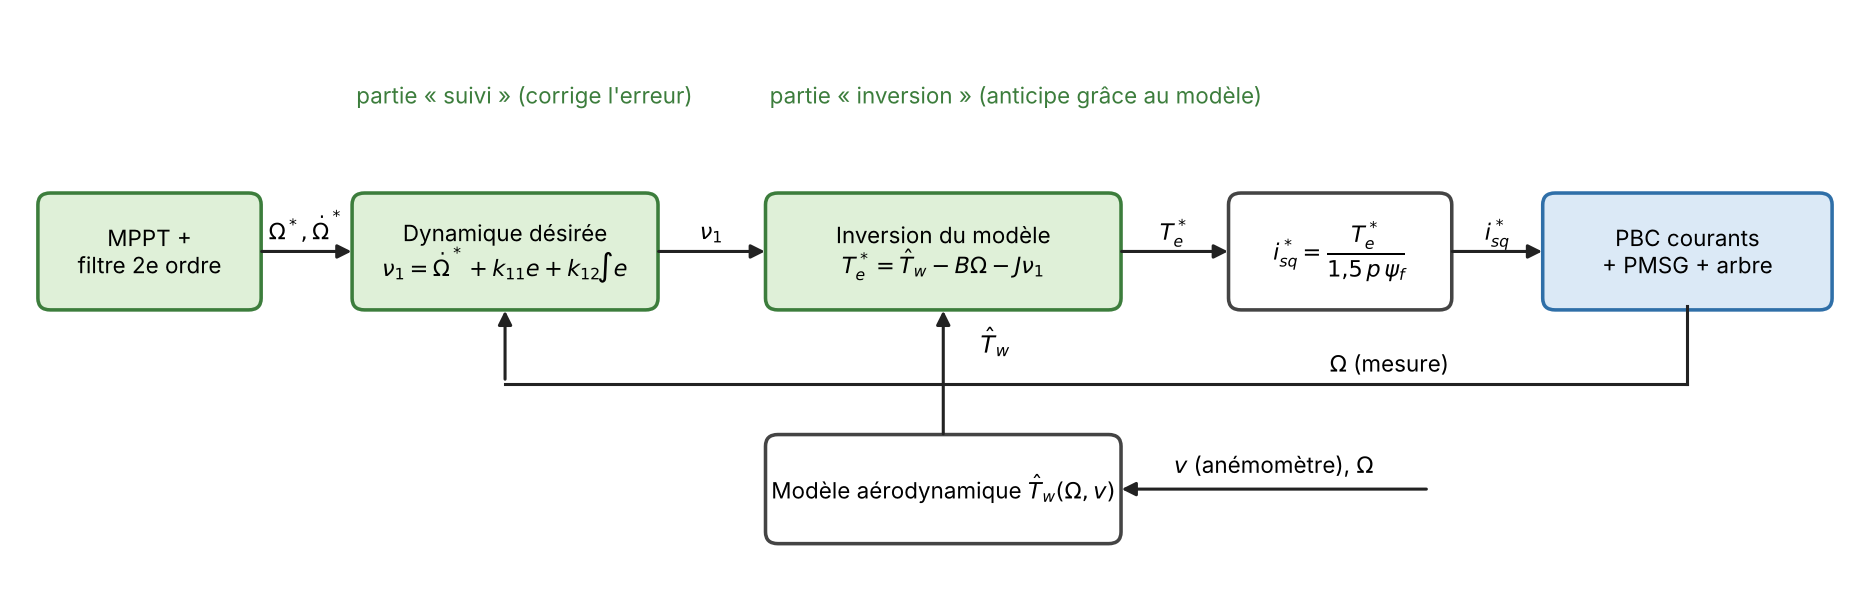
\includegraphics[width=\textwidth]{plat_schema.png}
\caption{Structure de la boucle de vitesse par platitude.}
\label{fig:schema}
\end{figure}

\begin{enumerate}
\item \textbf{Choisir la sortie plate} $y$ et vérifier qu'on peut exprimer la commande avec $y$ et ses dérivées.
\item \textbf{Construire la trajectoire de référence} $y^*(t)$, \emph{lisse}, avec ses dérivées
      ($\dot y^*$, parfois $\ddot y^*$).
\item \textbf{Imposer la dynamique désirée} : remplacer la dérivée $\dot y$ par
      \begin{equation}
      \nu = \dot y^* + k_1\, e + k_2\!\int\! e\,dt, \qquad e = y^* - y .
      \end{equation}
\item \textbf{Inverser le modèle} : calculer la commande avec $\nu$ à la place de $\dot y$.
\end{enumerate}

\paragraph{Pourquoi la forme de $\nu$ garantit-elle que l'erreur disparaît ?}
Si le modèle est exact, on obtient réellement $\dot y = \nu$. Alors
$\dot e = \dot y^* - \dot y = \dot y^* - \nu$, d'où :
\begin{equation}
\dot e + k_1\, e + k_2\!\int\! e\,dt = 0
\quad\Longleftrightarrow\quad
\ddot\varepsilon + k_1\dot\varepsilon + k_2\varepsilon = 0 \quad\text{avec}\quad \varepsilon=\int e\,dt .
\label{eq:erreur}
\end{equation}
C'est l'équation d'un \textbf{ressort avec amortisseur} : l'erreur revient à zéro toute seule. Son
équation caractéristique est $s^2 + k_1 s + k_2 = 0$. On la compare à la forme standard
$s^2 + 2\zeta\omega_n s + \omega_n^2 = 0$ :
\begin{equation}
\boxed{k_1 = 2\zeta\omega_n, \qquad k_2 = \omega_n^2}
\end{equation}
\begin{itemize}
\item $\omega_n$ (pulsation propre) fixe la \textbf{rapidité} : temps de réponse à 2\,\% $\approx 4/(\zeta\omega_n)$.
\item $\zeta$ (amortissement) fixe la \textbf{forme} : $\zeta=1$ sans dépassement, $\zeta=0{,}7$--$0{,}9$ un petit
      dépassement mais plus rapide.
\end{itemize}

\begin{figure}[h]
\centering
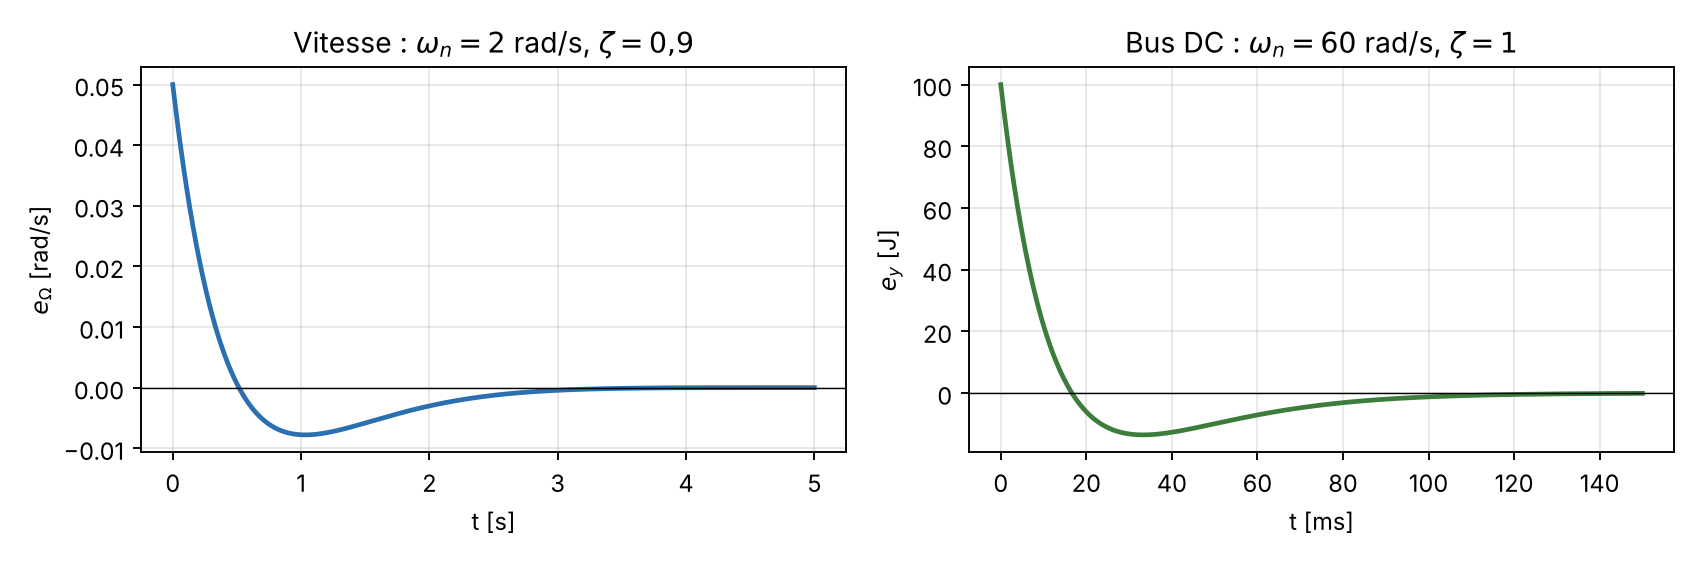
\includegraphics[width=\textwidth]{plat_erreur.png}
\caption{Disparition de l'erreur selon (\ref{eq:erreur}) avec les réglages choisis.
À gauche : boucle de vitesse (environ 2~s). À droite : boucle du bus (environ 70~ms).}
\label{fig:erreur}
\end{figure}

% =====================================================================
\section{Application 1 : la boucle de vitesse de la turbine}
% =====================================================================

\subsection{Étape 1 : la sortie plate est \texorpdfstring{$\Omega$}{Omega}}
Le modèle de l'arbre est
\begin{equation}
J\,\dot\Omega = T_w - T_e - B\,\Omega .
\label{eq:arbre}
\end{equation}
\begin{itemize}
\item État : $\Omega$. Commande : $T_e$ (le couple de la génératrice).
\item On choisit $y_1 = \Omega$. L'état est $\Omega = y_1$ : la condition 1 est vérifiée.
\item On inverse (\ref{eq:arbre}) : $T_e = T_w - B\,y_1 - J\,\dot y_1$. La commande s'écrit avec $y_1$ et
$\dot y_1$ : la condition 2 est vérifiée.
\end{itemize}
Le système est donc plat, de sortie plate $\Omega$. $T_w$ n'est pas un état : c'est une \textbf{entrée
extérieure} (une perturbation) qu'il faut connaître ou estimer.

\subsection{Étape 2 : la trajectoire de référence}
La MPPT donne la vitesse optimale $\Omega^*_{brut} = \lambda_{opt}\,v/R$. Mais on ne peut pas l'utiliser
directement :
\begin{itemize}
\item la mesure du vent $v$ est bruitée (anémomètre) ;
\item la platitude a besoin de la \textbf{dérivée} $\dot\Omega^*$, et dériver un signal bruité donne n'importe quoi.
\end{itemize}
On utilise donc deux filtres :
\begin{equation}
\tau_v\,\dot{\hat v} = v - \hat v \quad(\tau_v = 0{,}3~\text{s}),
\qquad
\ddot\Omega^* + 2\omega_r\,\dot\Omega^* + \omega_r^2\,\Omega^* = \omega_r^2\,\frac{\lambda_{opt}\,\hat v}{R}
\quad(\omega_r = 1{,}5~\text{rad/s}).
\end{equation}
Le filtre du second ordre est intéressant : en le calculant, on obtient \textbf{en même temps} $\Omega^*$ et
$\dot\Omega^*$, sans dériver numériquement. Dans le code (étape (a)) :
\begin{center}
\texttt{ddwr = G.wn\_ref\^{}2*(wraw - wr) - 2*G.wn\_ref*dwr;}\\ \texttt{wr = wr + Ts*dwr;\quad dwr = dwr + Ts*ddwr;}
\end{center}

\subsection{Étape 3 : la dynamique désirée}
\begin{equation}
\nu_1 = \dot\Omega^* + k_{11}\,e_\Omega + k_{12}\!\int\! e_\Omega\,dt, \qquad e_\Omega = \Omega^* - \Omega .
\end{equation}
\textbf{Choix des gains.} La turbine est très lourde ($J = 2{,}8\cdot10^6$~kg$\cdot$m$^2$) : inutile de
demander une réponse en 0,1~s, le couple nécessaire serait énorme. On prend $\omega_n = 2$~rad/s et
$\zeta = 0{,}9$ :
\begin{equation}
k_{11} = 2\times0{,}9\times2 = 3{,}6~\text{s}^{-1}, \qquad k_{12} = 2^2 = 4~\text{s}^{-2},
\qquad t_{r,2\%}\approx \frac{4}{0{,}9\times 2} \approx 2{,}2~\text{s}.
\end{equation}

\subsection{Étape 4 : l'inversion}
On remplace $\dot\Omega$ par $\nu_1$ dans $T_e = T_w - B\Omega - J\dot\Omega$. Comme $T_w$ n'est pas mesuré,
on le remplace par son estimation $\hat T_w$, calculée avec le modèle aérodynamique :
\begin{equation}
\hat T_w = \frac{\tfrac12\rho\pi R^2\,C_p(\lambda)\,v^3}{\Omega}, \qquad \lambda = \frac{\Omega R}{v},
\end{equation}
\begin{equation}
\boxed{T_e^* = \hat T_w - B\,\Omega - J\,\nu_1 \;(+\,\Delta T_e)}
\qquad\Longrightarrow\qquad
i_{sq}^* = \frac{T_e^*}{1{,}5\,p\,\psi_f}, \quad i_{sd}^* = 0 .
\end{equation}
Le terme $\Delta T_e$ vient du réseau de neurones ; on l'ignore ici (on le prend nul).

\paragraph{Lecture terme par terme.}
\begin{center}
\begin{tabular}{lp{11cm}}
\toprule
Terme & Rôle\\
\midrule
$\hat T_w$ & « La génératrice doit freiner autant que le vent pousse » : c'est l'équilibre (anticipation).\\
$-B\,\Omega$ & On freine un peu moins, car les frottements freinent déjà.\\
$-J\,\dot\Omega^*$ & Pour accélérer avec la référence, on freine moins (si $\dot\Omega^*>0$).\\
$-J\,k_{11}e_\Omega$ & Si la turbine est en retard ($e_\Omega>0$), on freine encore moins.\\
$-J\,k_{12}\int e_\Omega$ & Corrige les petites erreurs qui durent (modèle imparfait).\\
\bottomrule
\end{tabular}
\end{center}

\subsection{Exemple chiffré complet (un instant de la simulation)}
\begin{exemple}
\textbf{Situation :} vent $v = 8$~m/s ; la turbine tourne à $\Omega = 1{,}60$~rad/s ; la référence vaut
$\Omega^* = 1{,}62$~rad/s et augmente lentement, $\dot\Omega^* = 0{,}01$~rad/s$^2$ ; l'intégrale de l'erreur est nulle.
\begin{enumerate}
\item \textbf{Couple du vent estimé :}
      $\lambda = 1{,}60\times40/8 = 8{,}0$, d'où $C_p = 0{,}4798$ ;
      $P_w = 0{,}4798\times\tfrac12\times1{,}225\times\pi\times40^2\times8^3 = 0{,}756$~MW ;
      $\hat T_w = 0{,}756\cdot10^6/1{,}60 = 472{,}7$~kN$\cdot$m.
\item \textbf{Erreur :} $e_\Omega = 1{,}62 - 1{,}60 = 0{,}02$~rad/s (la turbine est en retard).
\item \textbf{Dynamique désirée :} $\nu_1 = 0{,}01 + 3{,}6\times0{,}02 + 4\times0 = 0{,}082$~rad/s$^2$.
\item \textbf{Couple de commande :}
      $T_e^* = 472{,}7 - \underbrace{1{,}6}_{B\Omega} - \underbrace{2{,}8\cdot10^6\times0{,}082/10^3}_{229{,}6} = 241{,}5$~kN$\cdot$m.
\item \textbf{Courant de référence :} $i_{sq}^* = 241\,500/(1{,}5\times26\times9{,}18) = 674$~A.
\end{enumerate}
\textbf{Interprétation :} à l'équilibre, il faudrait $471$~kN$\cdot$m (soit $1316$~A). Comme la turbine est en
retard, la commande freine \textbf{moitié moins} : le vent l'emporte et la turbine accélère. Quand
$\Omega$ rejoint $\Omega^*$, $T_e^*$ revient vers $471$~kN$\cdot$m.
\end{exemple}

\subsection{Et si le modèle est faux ? (pourquoi l'intégrale et l'ANN)}
Si $\hat T_w \neq T_w$, notons $\Delta = T_w - \hat T_w$. En injectant $T_e^*$ dans (\ref{eq:arbre}) :
\begin{equation}
J\dot\Omega = T_w - \hat T_w + J\nu_1 \quad\Longrightarrow\quad
\dot e_\Omega + k_{11}e_\Omega + k_{12}\!\int\! e_\Omega = -\frac{\Delta}{J}.
\end{equation}
\begin{itemize}
\item \textbf{Si $\Delta$ est constant :} en régime permanent $\dot e_\Omega = 0$ et $e_\Omega = 0$, donc
$\int e_\Omega = -\Delta/(J k_{12})$. L'intégrale \textbf{absorbe} l'erreur de modèle : la vitesse finit
quand même sur la référence.
\item \textbf{Si $\Delta$ varie} (il change avec le vent) : l'intégrale court toujours derrière, et une petite
erreur de vitesse subsiste. C'est exactement ce que le réseau de neurones corrige, en ajoutant
$\Delta T_e \approx \Delta$.
\end{itemize}
\begin{exemple}
Dans le test de robustesse, $\hat T_w$ est 10\,\% trop faible : $\Delta \approx 0{,}065$~MN$\cdot$m.
Alors $\Delta/J = 0{,}023$~rad/s$^2$ et l'intégrale se stabilise à $\int e_\Omega = -0{,}023/4 = -0{,}0058$~rad.
Avec l'ANN, $\Delta T_e \approx 0{,}065$~MN$\cdot$m compense directement $\Delta$ : l'erreur de vitesse
diminue de 39\,\%.
\end{exemple}

\subsection{Les saturations (anti-emballement)}
La génératrice ne peut pas fournir n'importe quel couple : $0 \le T_e \le 1{,}2\,T_n$ (pas de fonctionnement
moteur en MPPT). Si $T_e^*$ sort de ces limites, on le \textbf{limite}, et on \textbf{gèle l'intégrale}.
Sinon, pendant la saturation, l'intégrale grandirait inutilement et provoquerait ensuite un gros
dépassement (« emballement de l'intégrale », \emph{windup}).

% =====================================================================
\section{Application 2 : la boucle du bus continu}
% =====================================================================

\subsection{Étape 1 : pourquoi l'énergie est la bonne sortie plate}
\paragraph{Essai avec la tension.} L'équation du bus est
$C\,V_{dc}\,\dot V_{dc} = P_{msc} - P_{gsc}$, c'est-à-dire $\dot V_{dc} = (P_{msc}-P_{gsc})/(C\,V_{dc})$.
La tension apparaît au dénominateur : la relation est \textbf{non linéaire}, et l'inverser oblige à diviser
par $V_{dc}$.

\paragraph{Avec l'énergie.} On pose $W = \tfrac12 C V_{dc}^2$. Alors
$\dot W = C\,V_{dc}\,\dot V_{dc} = P_{msc} - P_{gsc}$ : c'est \textbf{linéaire}, un simple bilan
« entrée $-$ sortie ».

\paragraph{On ajoute l'énergie des bobines du filtre.} L'onduleur ne fournit pas directement la puissance
au réseau : il y a le filtre entre les deux, qui stocke aussi de l'énergie,
$W_L = \tfrac34 L_f\|\bv{i}_g\|^2$ (le facteur $\tfrac34$ vient de Park : $\tfrac12 L_f$ par phase $\times$
$\tfrac32$). Sa dérivée, avec l'équation du filtre
$L_f\dot{\bv{i}}_g = -R_f\bv{i}_g + \omega_g L_f\mathbf{J}\bv{i}_g + \bv{v}_i - \bv{v}_g$, vaut :
\begin{equation}
\dot W_L = \tfrac32\,\bv{i}_g^T L_f\dot{\bv{i}}_g
= -\tfrac32 R_f\|\bv{i}_g\|^2 + \underbrace{\tfrac32\omega_g L_f\,\bv{i}_g^T\mathbf{J}\bv{i}_g}_{=0}
+ \underbrace{\tfrac32\bv{v}_i^T\bv{i}_g}_{P_{gsc}} - \underbrace{\tfrac32\bv{v}_g^T\bv{i}_g}_{P_g}.
\end{equation}
En additionnant $\dot W + \dot W_L$, la puissance de l'onduleur $P_{gsc}$ \textbf{disparaît} :
\begin{equation}
\boxed{y_2 = \tfrac12 C V_{dc}^2 + \tfrac34 L_f\|\bv{i}_g\|^2, \qquad
\dot y_2 = P_{msc} - P_g - \tfrac32 R_f\|\bv{i}_g\|^2}
\end{equation}
avec $P_g = \tfrac32 v_{gd}\, i_{gd}$, la puissance réellement injectée au réseau. La commande
($i_{gd}$, à travers $P_g$) apparaît directement : $y_2$ est bien une sortie plate.

\subsection{Étapes 2 et 3 : référence et dynamique désirée}
La référence est constante : $y_2^* = \tfrac12 C V_{dc}^{*2} + \tfrac34 L_f\|\bv{i}_g^*\|^2$, donc
$\dot y_2^* \approx 0$. On impose $\dot y_2 = -\nu_2$ avec
\begin{equation}
\nu_2 = k_{21}\,e_y + k_{22}\!\int\! e_y\,dt, \qquad e_y = y_2^* - y_2 .
\end{equation}
\textbf{Choix des gains.} Le bus ne stocke que $14{,}4$~kJ : il doit réagir vite. On prend
$\omega_n = 60$~rad/s et $\zeta = 1$ :
\begin{equation}
k_{21} = 120~\text{s}^{-1}, \qquad k_{22} = 3600~\text{s}^{-2}, \qquad t_{r,2\%}\approx 4/60 \approx 70~\text{ms}.
\end{equation}

\subsection{Étape 4 : l'inversion}
De $\dot y_2 = P_{msc} - P_g - \tfrac32 R_f\|\bv{i}_g\|^2 = -\nu_2$, on tire la puissance à envoyer au réseau :
\begin{equation}
\boxed{P_g^* = P_{msc} - \tfrac32 R_f\|\bv{i}_g\|^2 - \nu_2 \;(+\,\Delta P_g)}
\qquad\Longrightarrow\qquad
i_{gd}^* = \frac{2P_g^*}{3\,v_{gd}}, \quad i_{gq}^* = 0 .
\end{equation}
\begin{itemize}
\item $P_{msc}$ : « renvoie au réseau tout ce que la génératrice fournit ». C'est l'\textbf{anticipation} :
      dès que la génératrice produit plus, l'onduleur envoie plus, avant même que la tension ne bouge.
      $P_{msc}$ est connu : $P_{msc} = \tfrac32(v_{sd}i_{sd}+v_{sq}i_{sq})$, avec les tensions appliquées et les
      courants mesurés.
\item $-\tfrac32 R_f\|\bv{i}_g\|^2$ : on retire les pertes du filtre.
\item $-\nu_2$ : la correction. Si l'énergie est trop basse ($e_y>0$), on envoie un peu moins au réseau
      pour recharger le bus.
\end{itemize}

\subsection{Exemple chiffré complet}
\begin{exemple}
\textbf{Situation :} la génératrice fournit $P_{msc} = 0{,}75$~MW ; la tension du bus est $V_{dc} = 1199$~V
($1$~V trop basse) ; $i_{gd} = 887$~A, $i_{gq} = 0$ ; $v_{gd} = 563{,}4$~V ; l'intégrale est nulle.
\begin{enumerate}
\item \textbf{Erreur d'énergie} (la partie du filtre est presque identique dans $y_2$ et $y_2^*$) :
      $e_y \approx \tfrac12\times0{,}02\times(1200^2 - 1199^2) = 24{,}0$~J.
\item \textbf{Correction :} $\nu_2 = 120\times24{,}0 = 2879$~W.
\item \textbf{Pertes du filtre :} $\tfrac32\times0{,}002\times887^2 = 2363$~W.
\item \textbf{Puissance à injecter :} $P_g^* = 750\,000 - 2363 - 2879 = 744\,758$~W.
\item \textbf{Courant de référence :} $i_{gd}^* = 2\times744\,758/(3\times563{,}4) = 881{,}3$~A.
\end{enumerate}
\textbf{Interprétation :} on envoie $2{,}9$~kW de moins que ce qui arrive. Ce surplus recharge le
condensateur, et la tension remonte vers $1200$~V en quelques dizaines de millisecondes.
\end{exemple}

\subsection{Comparaison avec un PI sur la tension}
Un PI classique calcule $i_{gd}^* = K_p(V_{dc}-V_{dc}^*) + K_i\int(V_{dc}-V_{dc}^*)$. Quand le vent augmente,
$P_{msc}$ augmente d'abord ; le PI ne réagit qu'\textbf{après} la montée de la tension. La loi plate, elle,
contient $P_{msc}$ : elle réagit \textbf{immédiatement}. C'est pourquoi, en simulation, $V_{dc}$ reste à
$\pm0{,}4$~V de $1200$~V en régime nominal.

% =====================================================================
\section{Récapitulatif}
% =====================================================================
\begin{center}
\begin{tabular}{p{3.2cm}p{6cm}p{6cm}}
\toprule
Étape & Boucle de vitesse & Boucle du bus continu\\
\midrule
1. Sortie plate & $y_1 = \Omega$ & $y_2 = \tfrac12 CV_{dc}^2 + \tfrac34 L_f\|\bv{i}_g\|^2$\\
Modèle & $J\dot\Omega = T_w - T_e - B\Omega$ & $\dot y_2 = P_{msc} - P_g - \tfrac32R_f\|\bv{i}_g\|^2$\\
2. Référence & $\Omega^*$, $\dot\Omega^*$ (MPPT + filtre) & $y_2^*$ constante, $\dot y_2^*\approx0$\\
3. Dynamique désirée & $\nu_1 = \dot\Omega^* + 3{,}6\,e + 4\!\int\!e$ & $\nu_2 = 120\,e_y + 3600\!\int\!e_y$\\
4. Inversion & $T_e^* = \hat T_w - B\Omega - J\nu_1$ & $P_g^* = P_{msc} - \tfrac32R_f\|\bv{i}_g\|^2 - \nu_2$\\
Vers les courants & $i_{sq}^* = T_e^*/(1{,}5\,p\psi_f)$ & $i_{gd}^* = 2P_g^*/(3v_{gd})$\\
Temps de réponse & $\approx 2{,}2$~s & $\approx 70$~ms\\
Correction ANN & $+\Delta T_e$ & $+\Delta P_g$\\
Dans le code & étape (b) & étape (d)\\
\bottomrule
\end{tabular}
\end{center}

\section{Questions fréquentes}
\begin{enumerate}
\item \textbf{Quelle différence entre platitude et PI ?}
Le PI ne connaît pas le système : il réagit à l'erreur. La platitude utilise le modèle pour calculer la
commande nécessaire \emph{avant} que l'erreur n'apparaisse, et garde une petite correction de type PI.

\item \textbf{Pourquoi a-t-on besoin de $\dot\Omega^*$ ?}
Parce que pour que la vitesse suive une référence qui change, il faut un couple d'accélération
$J\dot\Omega^*$. Sans ce terme, la vitesse serait toujours en retard.

\item \textbf{Pourquoi ne pas dériver $\Omega^*$ numériquement ?}
Parce que la dérivée d'un signal bruité est très bruitée. Le filtre du second ordre donne $\dot\Omega^*$
proprement.

\item \textbf{Pourquoi la boucle de vitesse est-elle lente (2~s) ?}
À cause de l'inertie énorme de la turbine : une réponse plus rapide demanderait des couples dépassant les
limites de la génératrice.

\item \textbf{Que se passe-t-il si le modèle $C_p$ est faux ?}
L'erreur de modèle agit comme une perturbation $-\Delta/J$. L'intégrale la compense si elle est constante.
Si elle varie, il reste une petite erreur, que l'ANN réduit.

\item \textbf{La boucle plate est-elle stable ?}
Avec le modèle exact, l'erreur suit (\ref{eq:erreur}), qui est stable pour $k_1, k_2 > 0$. Avec
$V = \tfrac12 e^2 + \tfrac12 k_2(\int e)^2$, on a $\dot V = -k_1 e^2 \le 0$.
\end{enumerate}

\end{document}
